\documentclass[spanish,a4paper,14pt,oneside]{extreport}

%%%%%%%%%%%%%%%%%%%%%%%%%%%%%%%%%%%%%%%%%%%%%%%%%%%%%%%%%%%%%%%%%%%%%%%%%%%%%%%
\usepackage[dvips]{graphicx}
\usepackage[dvips]{epsfig}
\usepackage[utf8]{inputenc}
\usepackage[spanish]{babel}
\usepackage{alltt}
\usepackage{algorithm}
\usepackage{algorithmic}
\usepackage{multirow}
\usepackage[top=2cm, bottom=2cm, left=2cm, right=2cm]{geometry}
%%%%%%%%%%%%%%%%%%%%%%%%%%%%%%%%%%%%%%%%%%%%%%%%%%%%%%%%%%%%%%%%%%%%%%%%%%%%%%%

\newcommand{\SONY}{{\sc Sony}}
\newcommand{\MICROSOFT}{{\sc Microsoft}}
\newcommand{\GCC}{\textsf{\textsc{G}CC}}
\newcommand{\INTEL}{\textsf{\textsc{I}ntel}}

%%% Traducimos el pseudocodigo
\renewcommand{\algorithmicwhile}{\textbf{mientras}}
\renewcommand{\algorithmicend}{\textbf{fin}}
\renewcommand{\algorithmicdo}{\textbf{hacer}}
\renewcommand{\algorithmicif}{\textbf{si}}
\renewcommand{\algorithmicthen}{\textbf{entonces}}
\renewcommand{\algorithmicrepeat}{\textbf{repetir}}
\renewcommand{\algorithmicuntil}{\textbf{hasta que}}
\renewcommand{\algorithmicelse}{\textbf{en otro caso}}
\renewcommand{\algorithmicfor}{\textbf{para}}

%\newcommand{\RETURN}{\textbf{retornar} }
\newcommand{\RET}{\STATE \textbf{retornar} }
\newcommand{\TO}{\textbf{hasta} }
\newcommand{\AND}{\textbf{y} }
\newcommand{\OR}{\textbf{o} }

%%%%%%%%%%%%%%%%% Creamos un entorno para listar código fuente %%%%%%%%%%%%%%%
\newenvironment{sourcecode}
{\begin{list}{}{\setlength{\leftmargin}{1em}}\item\scriptsize\bfseries}
{\end{list}}

\newenvironment{littlesourcecode}
{\begin{list}{}{\setlength{\leftmargin}{1em}}\item\tiny\bfseries}
{\end{list}}

\newenvironment{summary}
{\par\noindent\begin{center}\textbf{Abstract}\end{center}\begin{itshape}\par\noindent}
{\end{itshape}}

\newenvironment{keywords}
{\begin{list}{}{\setlength{\leftmargin}{1em}}\item[\hskip\labelsep \bfseries Keywords:]}
{\end{list}}

\newenvironment{palabrasClave}
{\begin{list}{}{\setlength{\leftmargin}{1em}}\item[\hskip\labelsep \bfseries Palabras clave:]}
{\end{list}}


%%%%%%%%%%%%%%%%%%%%%%%%%%%%%%%%%%%%%%%%%%%%%%%%%%%%%%%%%%%%%%%%%%%%%%%%%%%%%%%
% Format
%%%%%%%%%%%%%%%%%%%%%%%%%%%%%%%%%%%%%%%%%%%%%%%%%%%%%%%%%%%%%%%%%%%%%%%%%%%%%%%
%\usepackage{showframe}
%\marginparwidth 0mm
%%\topmargin -4 mm
%\topmargin -21 mm
%\headheight 10 mm
%\headsep 10 mm

%\textheight 229 mm
%\textheight 246 mm

%\oddsidemargin -5.4 mm
%\evensidemargin -5.4 mm
%\oddsidemargin 5 mm
%\evensidemargin 5 mm

%\oddsidemargin -3 mm
%\evensidemargin -3 mm

%\textwidth 17 cm
%\textwidth 15 cm
%\columnsep 10 mm

\input{amssym.def}

%%%%%%%%%%%%%%%%%%%%%%%%%%%%%%%%%%%%%%%%%%%%%%%%%%%%%%%%%%%%%%%%%%%%%%%%%%%%%%%

\begin{document}

%%%%%%%%%%%%%%%%%%%%%%%%%%%%%%%%%%%%%%%%%%%%%%%%%%%%%%%%%%%%%%%%%%%%%%%%%%%%%%%
% First Page
%%%%%%%%%%%%%%%%%%%%%%%%%%%%%%%%%%%%%%%%%%%%%%%%%%%%%%%%%%%%%%%%%%%%%%%%%%%%%%%

\pagestyle{empty}
\thispagestyle{empty}


\newcommand{\HRule}{\rule{\linewidth}{1mm}}
\setlength{\parindent}{0mm}
\setlength{\parskip}{0mm}

\vspace*{\stretch{0.5}}

\begin{center}

\includegraphics[scale=0.8]{images/logo_vertical}\\[10mm]
{\Huge Trabajo de Fin de Grado}
\end{center}

\HRule
\begin{flushright}
        {\Huge Título} \\[2.5mm]
        {\Large \textit{Title in English} .} \\[5mm]
        {\Large Autor} \\[5mm]


\end{flushright}
\HRule
\vspace*{\stretch{2}}
\begin{center}
  \Large La Laguna, \today
\end{center}

\setlength{\parindent}{5mm}

%%%%%%%%%%%%%%%%%%%%%%%%%%%%%%%%%%%%%%%%%%%%%%%%%%%%%%%%%%%%%%%%%%%%%%%%%%%%%%%
% Signature page (add the official stamp)
%%%%%%%%%%%%%%%%%%%%%%%%%%%%%%%%%%%%%%%%%%%%%%%%%%%%%%%%%%%%%%%%%%%%%%%%%%%%%%%
\newpage
%\cleardoublepage
\thispagestyle{empty}

D. {\bf Nombre Apellido1 Apellido2}, con N.I.F. 12.345.678-X
profesor
Titular de Universidad
adscrito al Departamento
de Nombre del Departamento
de la Universidad de La Laguna, como tutor

\bigskip
D. {\bf Nombre Apellido1 Apellido2}, con N.I.F. 12.345.678-X
profesor
Titular de Universidad
adscrito al Departamento
de Nombre del Departamento
de la Universidad de La Laguna, como cotutor

\bigskip
\bigskip
{\bf C E R T I F I C A (N)}

\bigskip
\bigskip
\bigskip
Que la presente memoria titulada:

\bigskip
``{\it Título del Trabajo.}''

\bigskip
\bigskip
\bigskip

\noindent ha sido realizada bajo su dirección por D. {\bf Nombre Apellido1 Apellido2},
con N.I.F. 12.345.678-X.

\bigskip
\bigskip

Y para que así conste, en cumplimiento de la legislación vigente y a los efectos
oportunos firman la presente en La Laguna a \today

%\cleardoublepage
\newpage
%%%%%%%%%%%%%%%%%%%%%%%%%%%%%%%%%%%%%%%%%%%%%%%%%%%%%%%%%%%%%%%%%%%%%%%%%%%%%%%
\thispagestyle{empty}

{ \flushright

\begin{LARGE}
Agradecimientos
\end{LARGE}

\hspace{3mm}

\begin{large}


\hspace{3mm}
XXX

\hspace{3mm}
XXX


\hspace{3mm}
XXX


\hspace{3mm}
XXX


\end{large}

}

%%%%%%%%%%%%%%%%%%%%%%%%%%%%%%%%%%%%%%%%%%%%%%%%%%%%%%%%%%%%%%%%%%%%%%%%%%%%%%%%%
\newpage

\begin{huge}
Licencia
\end{huge}

\bigskip
* Si NO quiere permitir que se compartan las adaptaciones de tu obra
y NO quieres permitir usos comerciales de tu obra indica:

\begin{center}

\includegraphics[scale=1.5]{images/by-nc-nd_88x31}\\[10mm]
{\Large \copyright~Esta obra está bajo una licencia de Creative Commons Reconocimiento-NoComercial-SinObraDerivada 4.0 Internacional.
}
\end{center}


\bigskip
* Si quiere permitir que se compartan las adaptaciones de tu obra mientras se comparta de la misma manera
y NO quieres permitir usos comerciales de tu obra indica:

\begin{center}

\includegraphics[scale=1.5]{images/by-nc-sa_88x31}\\[10mm]
{\Large \copyright~Esta obra está bajo una licencia de Creative Commons Reconocimiento-NoComercial-CompartirIgual 4.0 Internacional.
}
\end{center}



\bigskip
* Si quiere permitir que se compartan las adaptaciones de tu obra
y NO quieres permitir usos comerciales de tu obra indica:

\begin{center}

\includegraphics[scale=1.5]{images/by-nc_88x31}\\[10mm]
{\Large \copyright~Esta obra está bajo una licencia de Creative Commons Reconocimiento-NoComercial 4.0 Internacional.
}
\end{center}

\newpage

\bigskip
*Si NO quiere permitir que se compartan las adaptaciones de tu obra
y quieres permitir usos comerciales de tu obra indica:

\begin{center}

\includegraphics[scale=1.5]{images/by-nd_88x31}\\[10mm]
{\Large \copyright~Esta obra está bajo una licencia de Creative Commons Reconocimiento-SinObraDerivada 4.0 Internacional.
}
\end{center}


\bigskip
* Si quiere permitir que se compartan las adaptaciones de tu obra mientras se comparta de la misma manera
y quieres permitir usos comerciales de tu obra (licencia de Cultura Libre) indica:

\begin{center}

\includegraphics[scale=1.5]{images/by-sa_88x31}\\[10mm]
{\Large \copyright~Esta obra está bajo una licencia de Creative Commons Reconocimiento-CompartirIgual 4.0 Internacional.
}
\end{center}


\bigskip
* Si quiere permitir que se compartan las adaptaciones de tu obra
y quieres permitir usos comerciales de tu obra (licencia de Cultura Libre) indica:

\begin{center}

\includegraphics[scale=1.5]{images/by_88x31}\\[10mm]
{\Large \copyright~Esta obra está bajo una licencia de Creative Commons Reconocimiento 4.0 Internacional.
}
\end{center}



%%%%%%%%%%%%%%%%%%%%%%%%%%%%%%%%%%%%%%%%%%%%%%%%%%%%%%%%%%%%%%%%%%%%%%%%%%%%%%%
\newpage  %\cleardoublepage
\begin{abstract}
{\em

El objetivo de este trabajo ha sido ....
%
bla, bla, bla
%
bla, bla, bla
%
bla, bla, bla

\bigskip
La competencia [E6], que figura en la guía docente, indica que en la memoria del trabajo se ha de incluir:
antecedentes, problemática o estado del arte, objetivos, fases y desarrollo del proyecto,
conclusiones, y líneas futuras.


\bigskip
Se ha incluido el apartado de 'Licencia' con todas las posibles licencias abiertas (Creative Commons).
En el caso en que se decida hacer público el contenido de la memoria, habrá que elegir una de ellas
(y borrar las demás).
La decisión de hacer pública o no la memoria se indica en el momento de subir la memoria a la Sede Electrónica de la ULL, paso necesario en el proceso de presentación del TFG.

\bigskip
El documento de memoria debe tener un máximo de 50 páginas.

\bigskip
No se deben dejar páginas en blanco al comenzar un capítulo, ya que
el documento no está pensado para se impreso sino visionado
con un lector de PDFs.

\bigskip
También es recomendable márgenes pequeños ya que, al firmar digitalmente por
la Sede, se coloca un marco alrededor del texto original.


\bigskip
El tipo de letra base ha de ser de 14ptos.
}

\begin{palabrasClave}
Palabra reservada1, Palabra reservada2, ...
\end{palabrasClave}

\end{abstract}
%%%%%%%%%%%%%%%%%%%%%%%%%%%%%%%%%%%%%%%%%%%%%%%%%%%%%%%%%%%%%%%%%%%%%%%%%%%%%%%

%%%%%%%%%%%%%%%%%%%%%%%%%%%%%%%%%%%%%%%%%%%%%%%%%%%%%%%%%%%%%%%%%%%%%%%%%%%%%%%
\newpage  %\cleardoublepage
\begin{summary}
{\em

Here should be the abstract in a foreing language...

}

\begin{keywords}
Keyword1, Keyword2, Keyword3, ...
\end{keywords}

\end{summary}
%%%%%%%%%%%%%%%%%%%%%%%%%%%%%%%%%%%%%%%%%%%%%%%%%%%%%%%%%%%%%%%%%%%%%%%%%%%%%%%

%%%%%%%%%%%%%%%%%%%%%%%%%%%%%%%%%%%%%%%%%%%%%%%%%%%%%%%%%%%%%%%%%%%%%%%%%%%%%%%
\newpage{\pagestyle{empty}}
\thispagestyle{empty}

%%%%%%%%%%%%%%%%%%%%%%%%%%%%%%%%%%%%%%%%%%%%%%%%%%%%%%%%%%%%%%%%%%%%%%%%%%%%%%%


\pagestyle{myheadings} %my head defined by markboth or markright
% No funciona bien \markboth sin "twoside" en \documentclass, pero al
% ponerlo se dan un montón de errores de underfull \vbox, con lo que no se
% ha puesto.
\markboth{Nombre del alumno}{Título del proyecto}

%%%%%%%%%%%%%%%%%%%%%%%%%%%%%%%%%%%%%%%%%%%%%%%%%%%%%%%%%%%%%%%%%%%%%%%%%%%%%%%
%Numeracion en romanos
\renewcommand{\thepage}{\roman{page}}
\setcounter{page}{1}

%%%%%%%%%%%%%%%%%%%%%%%%%%%%%%%%%%%%%%%%%%%%%%%%%%%%%%%%%%%%%%%%%%%%%%%%%%%%%%%

\tableofcontents

%%%%%%%%%%%%%%%%%%%%%%%%%%%%%%%%%%%%%%%%%%%%%%%%%%%%%%%%%%%%%%%%%%%%%%%%%%%%%%%
\newpage{\pagestyle{empty}}

\listoffigures

%%%%%%%%%%%%%%%%%%%%%%%%%%%%%%%%%%%%%%%%%%%%%%%%%%%%%%%%%%%%%%%%%%%%%%%%%%%%%%%
\newpage{\pagestyle{empty}}

\listoftables

%%%%%%%%%%%%%%%%%%%%%%%%%%%%%%%%%%%%%%%%%%%%%%%%%%%%%%%%%%%%%%%%%%%%%%%%%%%%%%%
\newpage{\pagestyle{empty}}

%%%%%%%%%%%%%%%%%%%%%%%%%%%%%%%%%%%%%%%%%%%%%%%%%%%%%%%%%%%%%%%%%%%%%%%%%%%%%%%
%Numeracion a partir del capitulo I
\renewcommand{\thepage}{\arabic{page}}
\setcounter{page}{1}


\chapter{Introducción}
\label{chapter:intro}

%%%%%%%%%%%%%%%%%%%%%%%%%%%%%%%%%%%%%%%%%%%%%%%%%%%%%%%%%%%%%%%%%%%%%%%%%%%%%
% Chapter 1: Introducción 
%%%%%%%%%%%%%%%%%%%%%%%%%%%%%%%%%%%%%%%%%%%%%%%%%%%%%%%%%%%%%%%%%%%%%%%%%%%%%%%

%---------------------------------------------------------------------------------
\section{Introducción}
\label{1:sec:1}

En el área de arquitectura de computadores, es común repasar fundamentos teóricos
que tienen una base histórica y que resultan difíciles de comprender debido 
a que a pasar de que son las bases de los sistemas modernos, conllevan 
una gran abstracción respecto a las soluciones que se implementan en la actualidad.

\bigskip
En este trabajo, se hace hincapié en el aspecto del paralelismo a nivel de instrucción, 
un aparte fundamental de las computadoras modernas y que permitió una mejora exponencial
en el rendimiento.

\bigskip
Sin embargo, a pesar de que han pasado ya más de veinte años de los diseños iniciales,
este y muchos otros conceptos no resultan fáciles de enseñar en la docencia. A pesar de que 
todo es abstraíble a una serie de fundamentos simples, resulta muy difícil visualizar el 
paso de la \textit{segmentación} al paralelismo a nivel de instrucción.

\bigskip
En este contexto, un simulador permite ayudar a comprender, de manera visual y esquematizada
como funcionan estos mecanismos y actuar como un potente catalizador para la asimilación de los 
conceptos.


%---------------------------------------------------------------------------------
\section{Paralelismo a nivel de instrucción}
\label{1:sec:2}

El paralelismo a nivel de instrucción 

\subsection{Superescalar}


\subsection{VLIW}

Aunque no se desea entrar mucho en detalle en este aspecto, puesto que este trabajo de 
fin de grado se centra en la máquina superescalar, debe nombrarse la otra gran 
representante del paralelismo a nivel de instruccin, las máquinas \textit{Very Long Instruction Word}.

\bigskip
Mientras que las máquinas Superescalares hacen uso de un hardware complejo para llevar
a cabo el paralelismo a nivel de instrucción, las máquinas VLIW toman una vía opuesta.

\bigskip
El hardware se mantiene relativamente simple, y es el compilador, el que se encarga
de realizar las operaciones necesarias para permitir que se aproveche al máximo el 
paralelismo.

%---------------------------------------------------------------------------------
\section{Motivación para el trabajo}
\label{1:sec:3}

Como se ha mencionado, el uso de un simulador para apoyar la docencia de esta área
de Arquitecutra de Computadores resultaba un campo realmente interesante. De hecho,
esta herramienta ya existe. El actual profesor de la Universidad de La Laguna 
Iván Castilla desarrolló un simulador en C++ con este propósito.

\bigskip
Este simulador se ha estado utilizando como un complemento más de la docencia, pero
con el paso del tiempo, ha quedado obsoleto. No tanto por su funcionalidad, puesto
que los fundamentos teóricos sobre los que se basa no han cambiado con el tiempo, como 
por su aspecto visual y su accesibilidad.

\bigskip
Es por esto, se ha querido recuperar esta herramienta para continuar con su desarrollo 
y ampliación y este trabajo de fin de grado se centra en migrar esta aplicación a versión 
web de tal forma que sirva como base para los futuros proyectos.



%%%%%%%%%%%%%%%%%%%%%%%%%%%%%%%%%%%%%%%%%%%%%%%%%%%%%%%%%%%%%%%%%%%%%%%%%%%%%%%

\chapter{Título del Capítulo Dos}
\label{chapter:dos}

%%%%%%%%%%%%%%%%%%%%%%%%%%%%%%%%%%%%%%%%%%%%%%%%%%%%%%%%%%%%%%%%%%%%%%%%%%%%%%%
% Chapter 2: Antecedentes
%%%%%%%%%%%%%%%%%%%%%%%%%%%%%%%%%%%%%%%%%%%%%%%%%%%%%%%%%%%%%%%%%%%%%%%%%%%%%%%

%++++++++++++++++++++++++++++++++++++++++++++++++++++++++++++++++++++++++++++++

\section{SIMDE}
\label{2:sec1}
En el año dos mil cuatro, el por aquel entonces estudiante de esta universidad, 
Iván Castilla Rodríguez - y ahora tutor de este trabajo de fin de grado-, 
desarrolló como proyecto final de carrera un Simulador didáctico para la enseñanza 
de arquitectura de computadores, el cual fue bautizado como Simde. \cite{SIMDE}

\bigskip
Este simulador como se ha comentado en el apartado 1.4 cumple con las características
deseadas y esperadas de un simulador para la docencia de este ámbito.

\bigskip
Sin embargo, esta herramienta ya se encuentra desfasada. No ha sido un proyecto en constante
evolución, fue diseñada utilizando C++98 y C++ Builder y el código ahora mismo no resultaría
fácil de adaptar y mantener.

\begin{figure}[!th]
\begin{center}
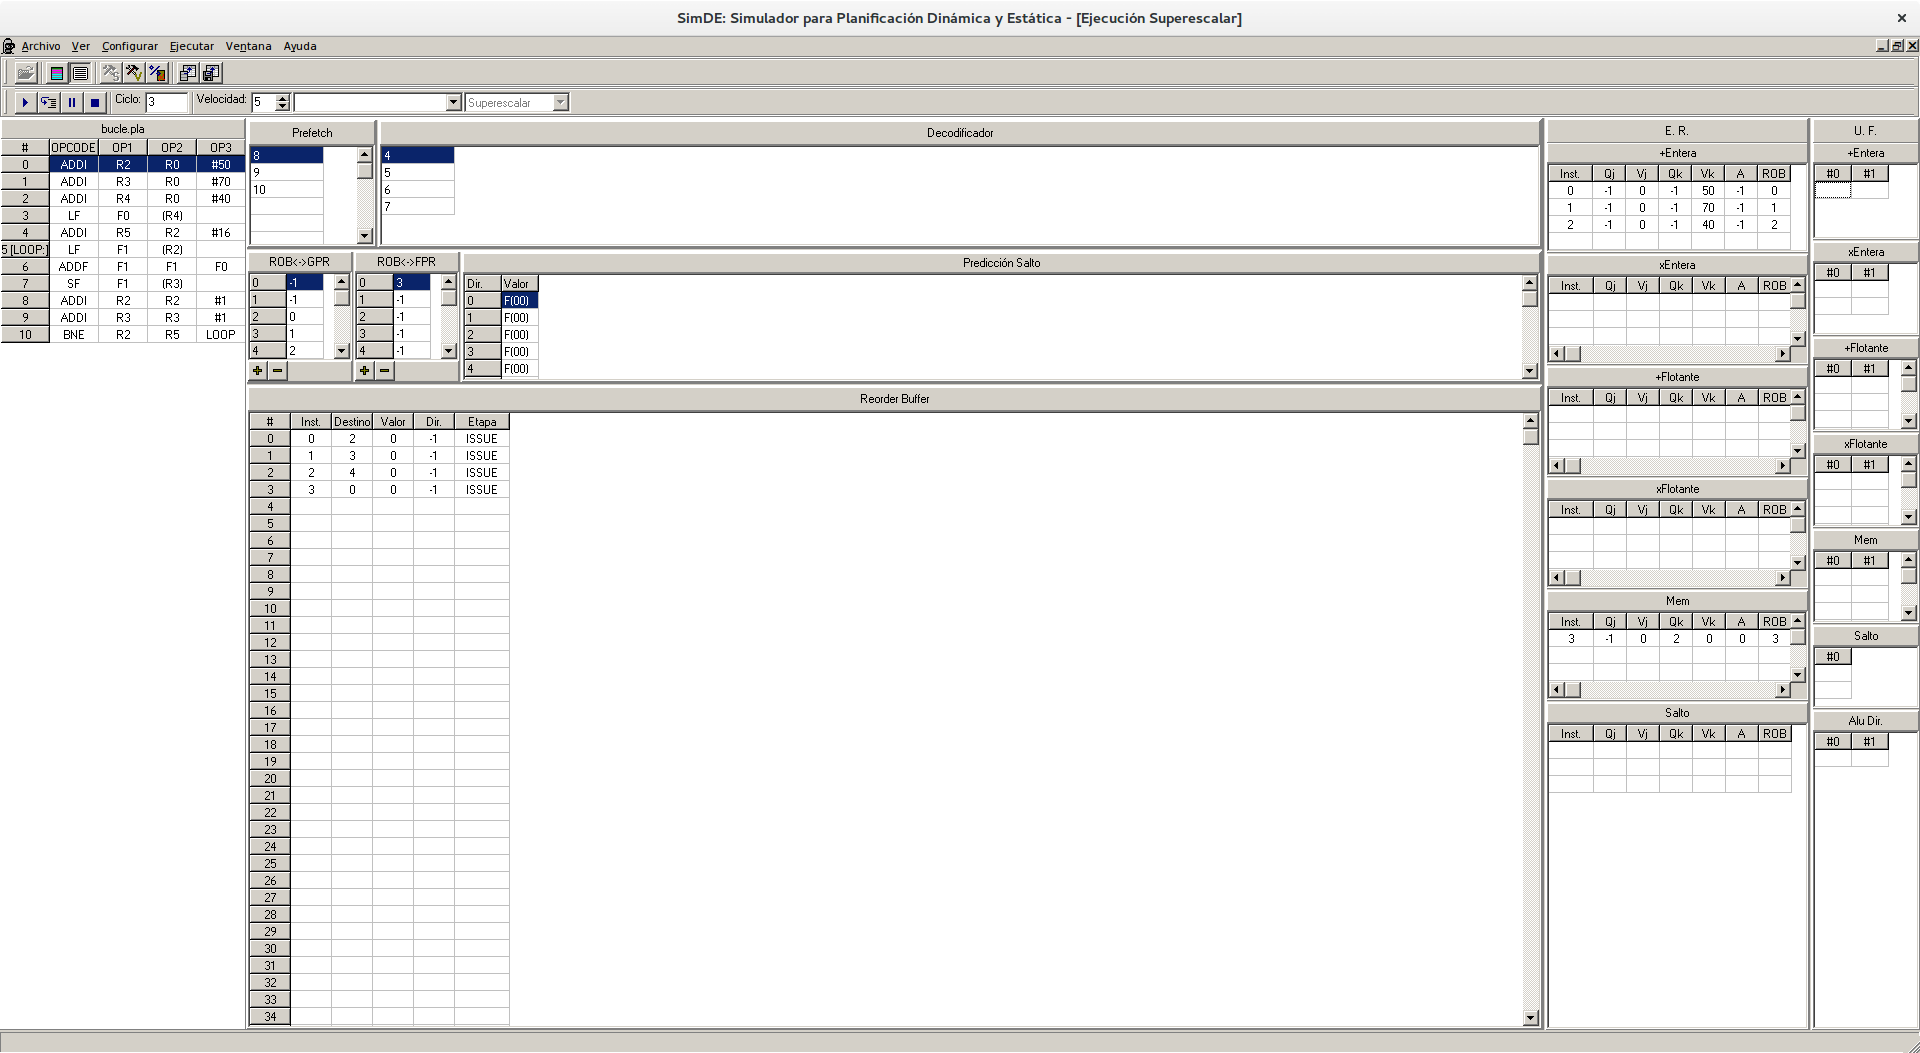
\includegraphics[width=0.8\textwidth]{images/cap2/simdeoriginal.eps}
\caption{Simulador original SIMDE}
\label{fig:Simulador original SIMDE}
\end{center}
\end{figure}

\section{Otros simuladores}
\label{2:sec2}
Sería irrazonable embarcarse en la tarea de migrar SIMDE sin comprobar antes si ya existe alguna
herramienta que se adapte a estas necesidades.

\begin{center}
    \begin{tabular}{| l | p{12cm} |}
    \hline
    Simulador & Descripción \\ \hline
    SESC & Simulador de máquinas Superescalares desarrollado en la Universidad de Illinois, posee
    características tan interesantes como el SMT, el CMP... Pero carece de interfaz gráfica. \\ \hline
    ReSIM & Este simulador de máquinas Superescalares está basado en la ejecución por trazas. Se encuentra 
    disponible para múltiples dispositivos Xilink. \\ \hline
    VLIW-DLX & Basado en WinDLX y desarrollado en la Universidad de praga, intenta aportar un conocimiento 
    detallado de las máquinas VLIW. \\ \hline
    \end{tabular}
\end{center}

Como vemos, aunque existen múltiples simuladores dentro de esta sección, ninguno cumple con el objetivo inicial,
es más, lamentablemente, la mayoría de los simuladores tienen más de una década y NINGUNO de los mencionados se 
encuentra disponible en versión web.

\section{Evolución del mundo web}
\label{2:sec3}
A modo de curiosidad, en el proyecto original, se consideraba poco factible la realización de 
un simulador de estas características en el entorno debido al escaso rendimiento. Cito textualmente:

\begin{quotation}
Utilizar programación web. Pese a las muchas ventajas de la programación
web en aspectos como la distribución y accesibilidad del programa, la realidad
es que el uso que se iba a dar a esta herramienta no invitaba a la utilización de
esta opción. El simulador no estaba planteado como una herramienta con
arquitectura cliente-servidor, ni tampoco se pretendía una ejecución distribuida.
La idea era que se procesara en la máquina del alumno y no en un servidor. El
uso de applets de java tampoco era una opción atractiva debido a la lentitud de
ejecución de java por ser interpretado.
\end{quotation} \cite{SIMDE}

\bigskip
Por sorprendete que resulte, este argumento totalmente justificado y válido en el momento
de su enunciado, resulta difícil de defender en un contexto actual. Hoy en día,
el rendimiento del lenguaje Javascript en el navegador es increíblemente alto. Y si vemos que la diferencia 
de este texto a ahora, es de unos escasos trece años -aunque ciertamenta nada despreciables en el mundo 
tecnológico, la diferencia resulta asombrosa.
 
\bigskip
Si intentamos encontrar un origen para esta diferencia tan increíble de rendimiento, sin duda
debemos remontar a la aparición de las primeras grandes aplicaciones que hacen uso de la tecnología
\textit{Ajax} como por ejemplo Gmail. La tendencia a diseñar más y más aplicaciones utilizando esta
tecnología resultó en una guerra por aumentar el rendimiento por parte de los distintos navegadores. \cite{EvolutionJavascript}





%%%%%%%%%%%%%%%%%%%%%%%%%%%%%%%%%%%%%%%%%%%%%%%%%%%%%%%%%%%%%%%%%%%%%%%%%%%%%%%
\newpage{\pagestyle{empty}}
\thispagestyle{empty}

\chapter{Título del Capítulo Tres}
\label{chapter:tres}

%%%%%%%%%%%%%%%%%%%%%%%%%%%%%%%%%%%%%%%%%%%%%%%%%%%%%%%%%%%%%%%%%%%%%%%%%%%%%%%
% Chapter 3: Tecnologías
%%%%%%%%%%%%%%%%%%%%%%%%%%%%%%%%%%%%%%%%%%%%%%%%%%%%%%%%%%%%%%%%%%%%%%%%%%%%%%%

%++++++++++++++++++++++++++++++++++++++++++++++++++++++++++++++++++++++++++++++
\section{Lenguaje para la lógica de la aplicación}
\label{3:sec1}

Por normal general cuando se habla de programación web en el lado del cliente, se tiende a pensar
de forma inmediata en Javascript, y en general, este razonamiento es totalmente válido. Pero dado que SIMDE
es una aplicación fuertemente orientada a objetos y con una gran base de código, se han valorado múltiples opciones.

\subsection{Coffescript}

\subsection{Dart}

Dart es un lenguaje de código abierto desarrollado por Google que permite desarrollador aplicaciones web, móvil, 
de servidor y también se puede utilizar en el \textit{Internet of Things}. 

\bigskip
Se ha considerado en el desarrollo de esta aplicación porque es un lenguaje orientado a objetos que utiliza una 
sintaxis similar a C\#. Además, aunque Google Chrome tiene una máquina virtual nativa para este lenguaje, es posible
transpilar el código a Javascript para los navegadores que no tiene este soporte nativo.

\begin{figure}[!th]
\begin{center}

\includegraphics[width=0.5\textwidth]{images/cap3/polymerlogo.eps}
\caption{Ejemplo}
\label{fig:PolymerLogo}
\end{center}
\end{figure}

Tras razonar detenidamente, Dart ha quedado descartado por diversas razones:

\begin{enumerate}
\item no va
\end{enumerate} 

\subsection{Typescript}

Typescript es un lenguaje libre y de código abierto desarrollado por Microsoft que actúa como un superconjunto
de Javascript, es decir incorpora los distintos estándares: ECMA5, ECMA6, ECMA7... Y además, como característica
destacable, añade comprobación de tipos en tiempo de compilación.

\bigskip
Este tipado no se refleja en el código final, de hecho una interfaz, por ejemplo,
añade 0 sobrecarga en el código final. Pero si que es interesante por las capacidades de
autocompletar (a través de Microsoft Intellisense)  que añade. Typescript se puede transpilar 
directamente a código javascript es5, el cuál es el estándar actual en todos los navegadores.    

\bigskip
Si tuviéramos que barajar una posible alternativa, sin duda la más destacada sería Flow, 
un comprobador de tipos para javascript desarrollado por Facebook. 

\bigskip
Pero existen múltiples razones para que haya escogido typescript sobre Flow:

\begin{enumerate}

\item Flow no está siendo parte de un proyecto de gran envergadura, se suponía que
 se introduciría en el desarrollo de react. Sin embargo no ha sido así.

\item Typescript es la opción de defacto para Angular 2, ha ido ganando mucho entusiasmo
 por parte de la comunidad y tiene un gran soporte.

\item Tengo cierta experiencia con Typescript.
\end{enumerate}

%++++++++++++++++++++++++++++++++++++++++++++++++++++++++++++++++++++++++++++++
\section{Tecnología para la integración modelo vista}
\label{3:sec2}

\subsection{Webcomponents}

Desde el inicio del proyecto, tenía claro que alguna librería se encargaría de realizar 
por mí el tedioso proceso de manipular el DOM. Actualmente existen múltiples librerías 
y frameworks que podían servirme en esta tarea, pero muchos de ellos (como por ejemplo Angular),
 no son lo suficientemente flexibles y acaban condicionando el desarrollo de la aplicación.

\bigskip
Lo que SIMDE necesitaba era un proyecto que hiciera uso de los Web components, 
una serie de apis que permiten crear etiquetas html personalizadas y reutilizables. 
Los webs componentes consisten en 4 características principales que pueden usarse 
por separado o todos juntos:

\begin{enumerate}

\item \textbf{Elementos personalizados.}
\item \textbf{Shadow DOM.}
\item \textbf{HTML Imports.}
\item \textbf{HTML Templates.}

\end{enumerate}

\subsection{Polymer}
Probablemente la librería basada en Web Componentes más conocida es Polymer,
una librería desarrollada por Google y anunciada en 2013. 

\bigskip

Pero a pesar de que las múltiples ventajas de Polymer existe una librería cuya comunidad es espléndida,
 y no es otra que React.

\subsection{React}
Existen una gran cantidad de motivos para escoger React sobre Polymer: Como por ejemplo, 
que ahora mismo se utiliza en decenas de aplicaciones importantes, como netflix, airbnb, Wallmart… (TODO INCLUIR CITA)

\bigskip
Que la comunidad es impresionantemente activa y cuenta con una gran cantidad de usuarios dispuestos a ayudar, así como cuenta con muchísima documentación y muchísimas implementaciones de librerías de terceros.

\bigskip
React utiliza un híbrido entre html y javascript denominado jsx, como también tiene soporte para 
Typescript, en este caso utilizamos tsx, y se basa en un “unidirectonial data-flow”. 

\bigskip
Ademas React implementa operaciones sobre el DOM virtual de tal forma que las operaciones sobre
el verdadero DOM sean eficientes.

%++++++++++++++++++++++++++++++++++++++++++++++++++++++++++++++++++++++++++++++
\section{Tecnología para hacer la build}
\label{3:sec3}

\subsection{Gulp/Grunt}

\subsection{Webpack}
\bigskip
Una de las grandes herramientas de 2016 que acabó por cambiar el flujo de muchos 
desarrolladores web y desbancó a tasks runners como Grunt y Gulp fue webpack.

\bigskip
Para poder integrar todo este código y resolver el problema de los múltiples imports 
era necesario utilizar algún tipo de herramienta de gestión de paquetes, como por ejemplo 
commonjs, o requirejs. Sin embargo, webpack se encarga de resolver todas estas 
dependencias y crear statics assets para el navegador.

\bigskip
Uno de los mayores puntos a favor es que es altamente configurable, existen muchísimos 
plugins de webpack que permiten hacer preprocesamiento de css, tratamiento de imágenes,
minimización codigo, étctera.. 

\bigskip
Actualmente en la aplicación de SIMDE webpack  se encarga de compilar el código de 
typescript, el código de react y de generar un bundle 

%++++++++++++++++++++++++++++++++++++++++++++++++++++++++++++++++++++++++++++++
\section{Tecnología para la documentación}
\label{3:sec4}

Para integrar la documentación en la nueva aplicación web de SIMDE resultaba obvio que esta documentación
estuviera también en formato web. Para esto existían muchas alternativas, desde un conjunto de ficheros
html hasta un pequeño cms. 

Dado que la documentación es bastante extensa pero que en realidad, no es mas que un documento 
que se redactará en una ocasión y se le irán realizando pequeñas ampliaciones y/o correcciones
se optó por una solución diferente, los generadores de contenido estático.

\subsection{Generadores de contenido estático}

Los gneeradores de contenido estático 

\subsection{Hexo}





%%%%%%%%%%%%%%%%%%%%%%%%%%%%%%%%%%%%%%%%%%%%%%%%%%%%%%%%%%%%%%%%%%%%%%%%%%%%%%%

\chapter{Título del Capítulo Cuatro}
\label{chapter:cuatro}

%%%%%%%%%%%%%%%%%%%%%%%%%%%%%%%%%%%%%%%%%%%%%%%%%%%%%%%%%%%%%%%%%%%%%%%%%%%%%%%
% Chapter 4: Tecnologías
%%%%%%%%%%%%%%%%%%%%%%%%%%%%%%%%%%%%%%%%%%%%%%%%%%%%%%%%%%%%%%%%%%%%%%%%%%%%%%%

Uno de los puntos más importantes de este trabajo era determinar las diferentes tecnologías
a utilizar. El mundo web ha sufrido una gran revolución en los últimos años y ahora
se disfruta de una gran variedad de propuestas para cada tipo de tarea.

Es por ello, que ha habido que hacer una gran valoración del estado del arte 
tecnológico para determinar qué curso debería seguir la aplicación.

%++++++++++++++++++++++++++++++++++++++++++++++++++++++++++++++++++++++++++++++
\section{Lenguaje para la lógica de la aplicación}
\label{4:sec1}
Por normal general cuando se habla de programación web en el lado del cliente, se tiende a pensar
de forma inmediata en Javascript, y en general, este razonamiento es indudablemente válido. 
Pero dado que SIMDE es una aplicación fuertemente orientada a objetos y con una gran base de código, 
se han valorado múltiples alternativas con el objetivo de agilizar la realización de este proyecto.

\subsection{Coffescript}

Coffescript es un pequeño lenguaje que se compila en Javascript, su objetivo era mejorar la legibilidad 
y concisión de Javascript añadiendo varios \textit{syntactic sugars} inspirados en otros lenguajes como
\textit{Ruby} o \textit{Python}. \cite{Coffescript}

\bigskip
Coffescript es un lenguaje con un largo recorrido, apareciendo a finales del año 2009. Y tiene soporte por
parte de \textit{Ruby on Rails} y \textit{Play framework}. \cite{CoffescriptWiki}

\bigskip 
Coffescript podría ser la opción ideal para agilizar le desarrollo debido a la similitud de sintaxis con 
Ruby.

\begin{lstlisting}
class Animal
  constructor: (@name) ->

  alive: ->
    false

class Parrot extends Animal
  constructor: ->
    super("Parrot")

  dead: ->
    not @alive()
\end{lstlisting}

\bigskip
Sin embargo, la opción de Coffescript ha sido desestimada en gran medida por su decreciente popularidad
y la poca certeza del futuro que tomará el lenguaje.

\subsection{Dart}

Dart es un lenguaje de código abierto desarrollado por Google que permite desarrollador aplicaciones web, móvil, 
de servidor y también se puede utilizar en el \textit{Internet of Things}. \cite{Dart}

\bigskip
Se ha considerado en el desarrollo de esta aplicación porque es un lenguaje orientado a objetos que utiliza una 
sintaxis similar a C\#. Además, aunque Google Chrome tiene una máquina virtual nativa para este lenguaje, es posible
transpilar el código a Javascript para los navegadores que no tiene este soporte nativo.

\bigskip
Tras razonar detenidamente, ha pesar de lo atractivo del lenguaje, Dart ha quedado descartado por 
una razón de peso y es que se trata de un lenguaje totalmente diferente y su uso es mayoritariamente
por parte de Google.

\subsection{Typescript}

Typescript es un lenguaje libre y de código abierto desarrollado por Microsoft que actúa como un superconjunto
de Javascript, es decir incorpora los distintos estándares: ECMA5, ECMA6, ECMA7... Y además, como característica
destacable, añade comprobación de tipos en tiempo de compilación. \cite{Typescript}

\bigskip
Este tipado no se refleja en el código final, de hecho una interfaz, por ejemplo,
añade 0 sobrecarga en el código final. Pero si que es interesante por las capacidades de
autocompletado (a través de Microsoft Intellisense)  que añade.

\begin{figure}[!th]
\begin{center}
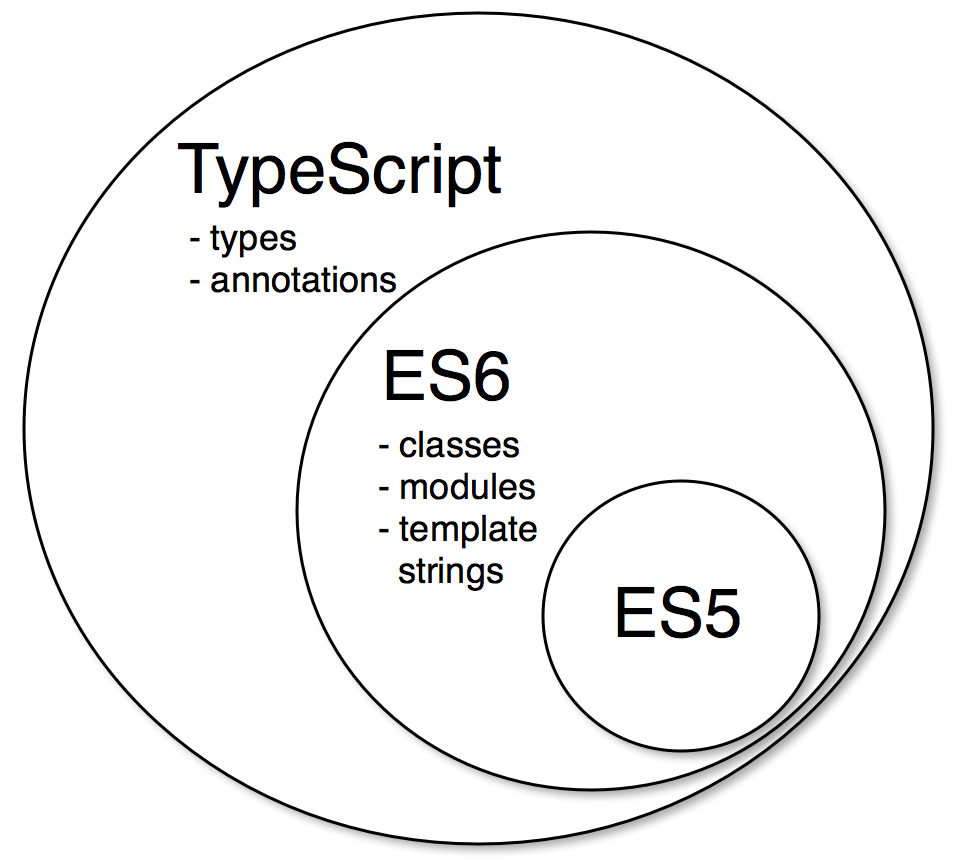
\includegraphics[width=0.5\textwidth]{images/cap4/typescript.eps}
\caption{Typescript como superconjunto de Javascript}
\label{fig:Typescript como superconjunto de Javascript}
\end{center}
\end{figure}

\bigskip
Al final, en este proyecto Typescript ha sido la tecnología ganadora, y existen múltiples
razones:

\begin{enumerate}

\item Typescript tiene bastante apoyo por parte de la comunidad y por parte de la propia Microsoft.
La documentación es extensa y efectiva.

\item Typescript está alineada en cierta forma con el futuro de Javascript. Microsoft es uno de los 
muchos que forman parate del concenso de estándar de ECMASCRIPT.

\item Typescript no me limita en la posibilidad de usar javascript, todo código javascript es código
Typescript válido.

\item Por último y no menos importante: Tengo cierta experiencia con Typescript.
\end{enumerate}



%++++++++++++++++++++++++++++++++++++++++++++++++++++++++++++++++++++++++++++++
\section{Tecnología para la integración modelo vista}
\label{4:sec2}
Desde el inicio del proyecto, se tenía claro que alguna librería se encargaría de gestionar
 el tedioso proceso de manipular el DOM. Actualmente existen múltiples librerías 
y frameworks que podían servir para realizar esta tarea, pero muchos de ellos (como por ejemplo Angular),
son demasiado \textit{rígidos} y acaban condicionando la forma de desarrollar la aplicación, 
lo cual resulta ser contraproducente.

\subsection{Webcomponents}

\bigskip
Una de las características más deseadas para el nuevo diseño de la interfaz de SIMDE era contar con
un diseño basado en componentes. Siendo la caracteŕistica más deseada de todo el incorporar las nuevas 
ventajas que ofrecen los \textit\textbf{Web Components}. Los Web Components son un conjunto de 
características que se están añadiendo a las especificaciones W3C de Html y del DOM. \cite{Webcomponents}

\bigskip 
El objetivo de estas características es permitir crear componentes personalizados, reusables y 
con su propia encapsulación. Esto se consigue a través de cuatro características principales:

\begin{enumerate}

\item \textbf{Elementos personalizados}: Esta característica permite diseñar y utilizar nuevos tipos 
de elementos del DOM.
\item \textbf{Shadow DOM}: Esta característica permite al navegador incluir un subarbol de elementos del 
DOM en el renderizado del documento pero \textbf{NO} se incluyen el DOM principal.
\item \textbf{HTML Imports}: Esta característica permite incluir y reutilizar documentos HTML en otros 
documentos HTML.
\item \textbf{Plantillas HTML}: Esta característica permite declarar fragmentos de código de marcas que no
se utilizan en el carga de la página pero que se pueden instanciar en tiempo de ejecución. 

\end{enumerate}

\subsection{Polymer}
Esta librería fue la primera que hizo uso de los Web Components.Desarrollada por Google y anunciada en 
el año 2013, Polymer permite aprovechar las características de los Web Components \cite{Polymer} a través de los polyfills 
-códigos que implementan características en los navegadores que no soportan las mismas de forma nativa-.
\textit{(Comúnmente se conoce como polyfill a la librería que implementa el estándar de HTML5)}. \cite{Polyfill} 

\bigskip
A pesar de la revolución que marcó, Polymer no fue ampliamente acogida por la comunidad de desarrolladores 
-quizás por ser una librería adelantada a su tiempo-. Y hoy en día nos encontramos con otro intento por 
parte de ganar peso en la comunidad: Polymer 2.0. Esta nueva versión incorpora el soporte de las clases de ES6
y además permite utilizar el método de la especificación de custom elements v1 para definir elementos.

\bigskip
Aunque las mejoras que incorpora Polymer 2.0 la hacen una opción totalmente válida y viable, aún no 
tiene una comunidad lo suficientemente sólida con lo que esto acaba traduciéndose en una menor 
cantidad de recursos disponibles.

\subsection{React}
La empresa autora de esta librería de código abierto, Facebook, la define como: “It’s a Javascript library for building UI’s”. \cite{React}

\bigskip
Pero realmente aunque esta declaración es totalmente cierta, React no es tan algo tan simple. Para resolver el problema
 de la modificación del DOM de una forma eficiente: Simulándolo esta estructura en memoria y aplicando diversos
 algoritmos para calcular cuales serían los mínimos cambios necesarios a realizar sobre el \textit{DOM verdadero}
 para representar los diversos cambios de estado.

\bigskip
React se basa en el uso de componentes, no en el sentido explícito de los \textit{Web Components} tal como los define 
el éstandar de HTML5, sino como pequeños bloques reusables que incorporan cierta funcionalidad. Sin embargo, a pesar 
de que React se puede integrar con la api de \textit{Web Components}, el uso de esta api incrementa de forma exponencial
la complejidad de la aplicación, con lo cual se ha pospuesto el uso de esta característica para versiones futuras.


\bigskip
React utiliza un híbrido entre html y javascript denominado jsx, como también tiene soporte para 
Typescript, en este caso utilizamos tsx.

\begin{figure}[!th]
\begin{center}
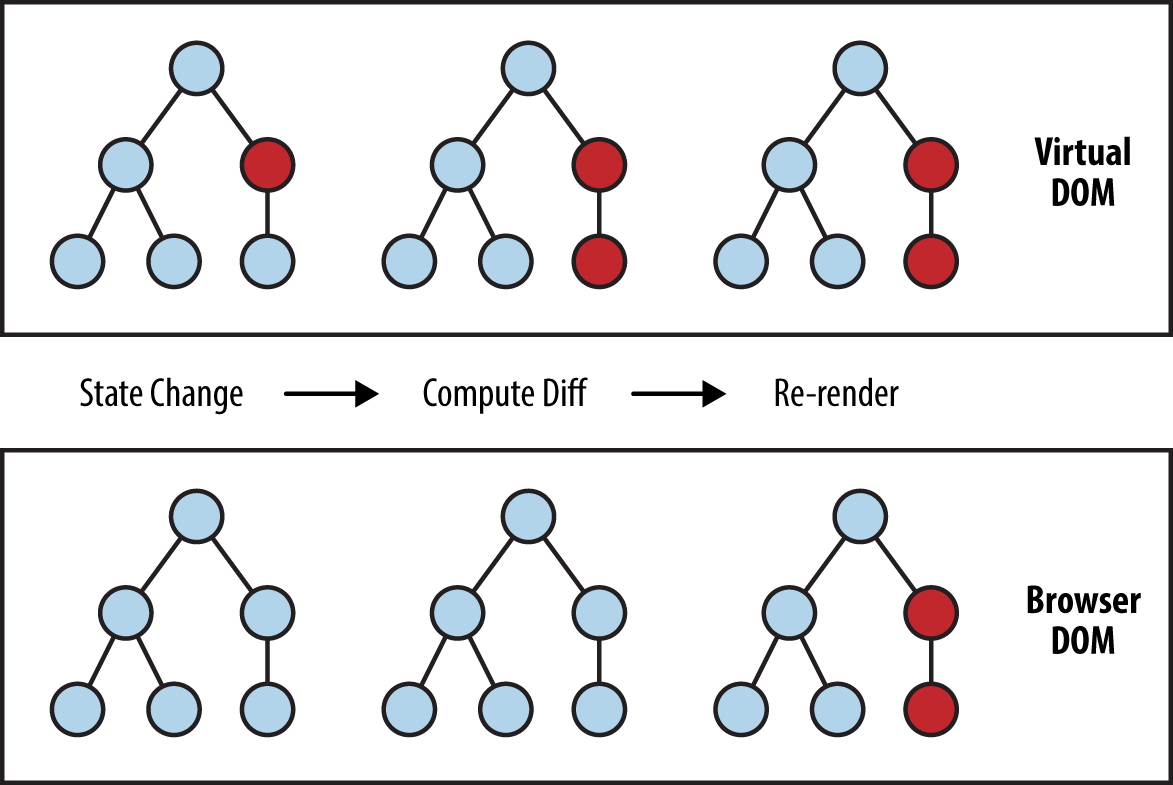
\includegraphics[width=0.8\textwidth]{images/cap4/react-virtual-dom.eps}
\caption{Funcionamiento del DOM virtual de React \cite{ReactVirtualDOM}}
\label{fig:Funcionamiento del DOM virtual de React}
\end{center}
\end{figure}

\bigskip
React es ampliamente utilizada por muchísimas empresas gracias a su capacidad de integrarse con otras librerías. 
Por ejemplo Microsoft mantuvo parte de la página en jQuery mientras iba integrando React.

\bigskip
Otro ejemplo de grandes empresas que hagan uso de esta librería son: AirBnB, Netflix, Wallmart…  \cite{ReactUsers}

\bigskip
Y muchas de ellas han contribuido al ecosistema de React, ya sea mediante guías de estilo, conjunto de componentes, patrones... \cite{ReactStyleGuide}

\bigskip
Además,la comunidad de usuarios es increíblemente activa, por ejemplo es común ver a Dan Abramov resolviendo dudas
en distintos sitios como \textit{Github} o \textit{Reddit}. Dan Abramov es el creador de Redux (una implementación de gestión de estados), desarrollador de la nueva implementación de 
React \textit{(react-fiber)}, empleado de Facebook, participante en muchas conferencias y además autor de 
múltiples herramientas como \textit{react-hot-loader}. 

\bigskip
Debido a todo lo anterior y a que además, React tiene una excelente integración con Typescript utilizando 
el formato .tsx, queda claro que es la mejor opción posible para esta aplicación. React es una librería 
desarrollada por Facebook para construir interfaces.


%++++++++++++++++++++++++++++++++++++++++++++++++++++++++++++++++++++++++++++++
\section{Tecnología para hacer la build}
\label{4:sec3}
Debido a la complejidad de las aplicaciones web modernas, es necesario 
realizar una serie de pasos intermedios entre el código original y 
el resultado final de la apliación. Para el caso de este proyecto, se debe:

\begin{itemize}

\item Compilar el código typescript a javascript.

\item Compilar el código .tsx a .jsx.

\item Resolver las importaciones de dependencias, tanto de la lógica
como de los componentes.

\item Procesar el código sass y convertirlo en css.

\end{itemize}

\subsection{Gulp/Grunt}

La primera tendencia -debido a su gran extensión- sería utilizar 
lo que se conoce como un \textit{task runner}. Actualmente, dos de los 
más conocidos son \textbf{Grunt} \cite{grunt} y  \textbf{Gulp} \cite{gulp}.

\bigskip
Ambos están basados en NodeJs y son compatibles entre sí en gran medida.
Su funcionamiento es sencillo, en un gruntfile o gulpfile se definen las tareas a
ejecutar, seleccionando los ficheros de fuente sobre los que actuar -si cabe- y la tarea 
a realizar.

\bigskip
Existen muchisimos plugins desarrollados que permiten hacer todo tipo de tareas, desde traducir
markdown hasta minimizar el contenido de los ficheros de estilos y de javascript.

\bigskip
Sin embargo, a pesar de que esta opción era altamente atractiva debido 
a su robustez, se ha optado por probar una solución aún más moderna, \textbf{webpack}.

\subsection{Webpack}

Webpack es un \textit{empaquetador de módulos} para aplicaciones de Javascript modernas.
Cuando webpack procesa la aplicación, construye un grafo de dependencias
incluyendo todos los módulos y luego lo empaqueta en orden \cite{webpack}.  

\bigskip
Webpack incorpora de serie diversas características interesantes tales como el 
poder ejecutar un servidor de desarrollo que aplica \textit{hot reloading} sobre el código 
sin requerir refrescar la página o el poder separar el código css/js de terceros para el 
entorno de producción. 

\bigskip 
El funcionamiento de webpack puede ser extremadamente resumido y simplificado en:

\begin{itemize}

\item Partiendo de un punto de entrada, una serie de reglas sobre los distintos tipos de ficheros
activan una serie de \textit{loaders} correspondientes para procesarlos. 

\item Estos loaders pueden ser concatenados entre sí para obtener el resultado deseado, por ejemplo
podemos traducir el código typescript a es6 para luego traducir este código junto a otro a es5 mediante
babel.

\item Se aplican, si fuera necesario, el uso de plugins para tareas más complejas que se quieren aplicar sobre
todos los paquetes.

\end{itemize}

\begin{figure}[!th]
\begin{center}
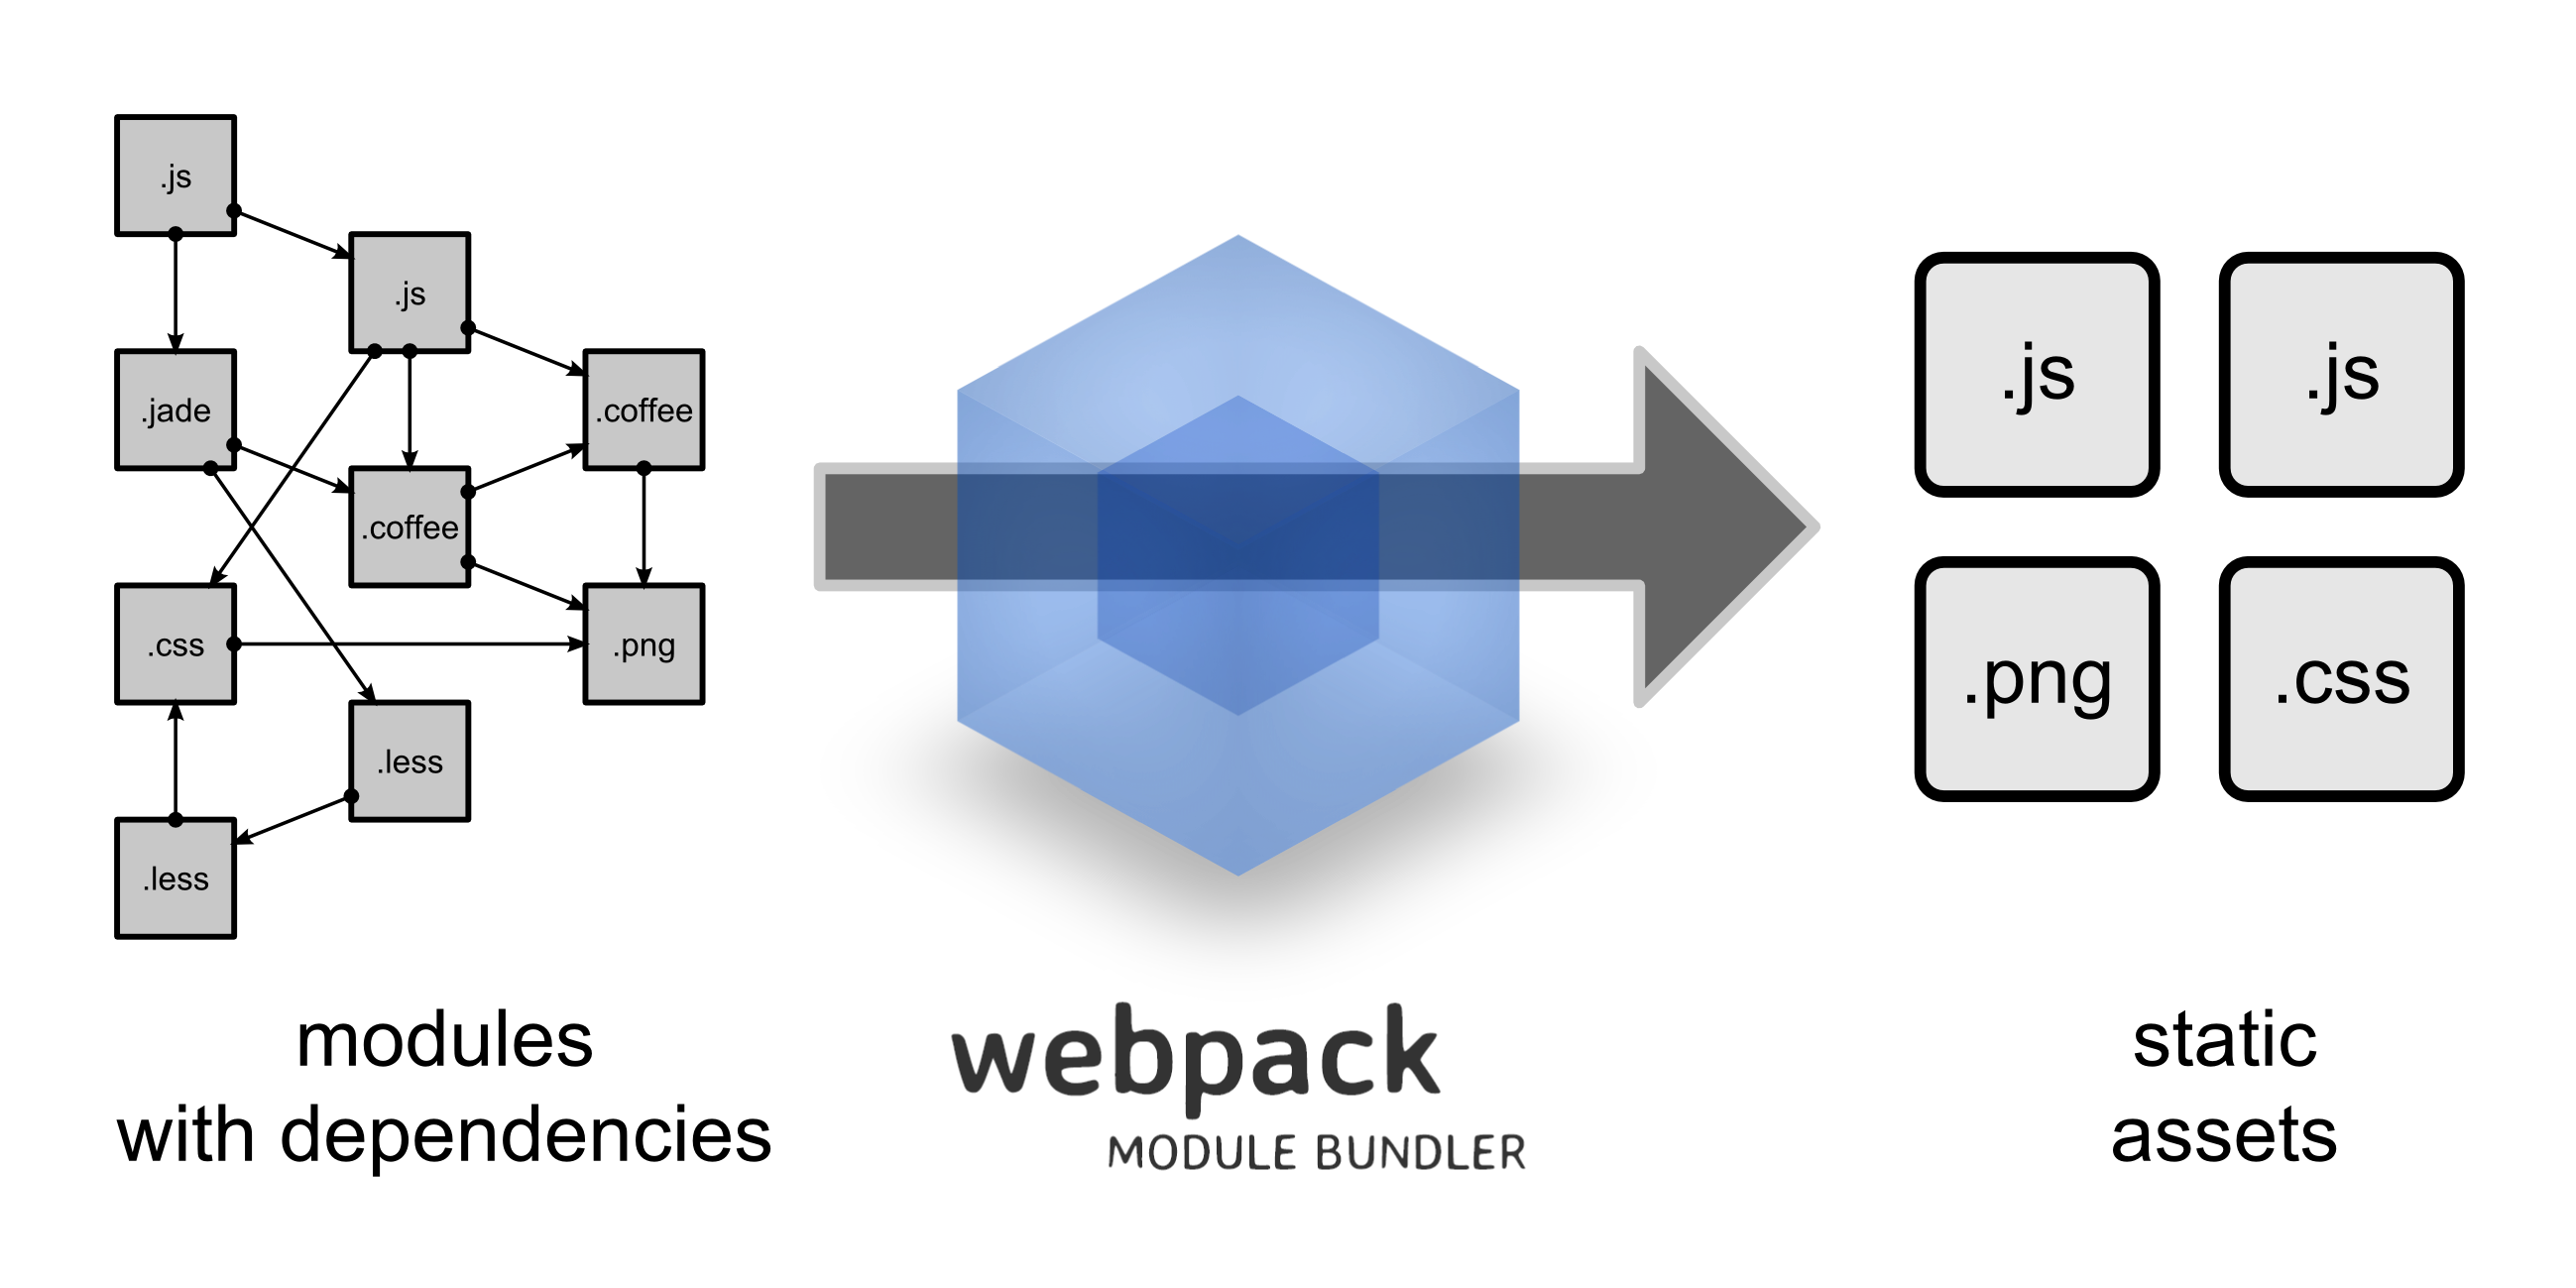
\includegraphics[width=0.8\textwidth]{images/cap4/webpack.eps}
\caption{Imagen descriptiva de Webpack}
\label{fig:Imagen descriptiva de Webpack}
\end{center}
\end{figure}


Como resultado final se obtiene una serie de paquetes que contienen todas las dependencias resueltas.

%++++++++++++++++++++++++++++++++++++++++++++++++++++++++++++++++++++++++++++++
\section{Tecnología para la documentación}
\label{4:sec4}
Para integrar la documentación en la nueva aplicación web de SIMDE resultaba obvio que esta documentación
estuviera también en formato web. Para esto existían muchas alternativas, desde un conjunto de ficheros
html hasta un pequeño sistema de gestión de contenidos. 

\bigskip
Dado que la documentación es bastante extensa pero que en realidad, no es más que un documento 
que se redactará en una ocasión y se le irán realizando pequeñas ampliaciones y/o correcciones
se optó por una solución diferente, los generadores de contenido estático.

\subsection{Generadores de contenido estático}

Los generadores de contenido estático se encargan -resumido de forma tosca y breve- de generar 
un conjunto de htmls y css a partir de una plantilla y una serie de ficheros fuentes. 

\bigskip
Este tipo de generadores estáticos tienen un gran auge entre los desarrolladores que desean 
mantener un blog -yo mismo por ejemplo, tengo uno hecho en Hugo-. 

\bigskip 
Existen múltiples ventajas de utilizar este tipo de tecnologías, pero sin duda para mi la más
importante, es que se alimentan de un formato como es el markdown. El cual es muy intuitivo de 
usar y tiene soporte más allá de este tipo de tecnologías. 

\subsection{Hexo}

Hexo es un generador de contenido estático basado en NodeJS. No posee demasiadas diferencias destacables
sobre el resto de alternativas, y ha sido escogido para este proyecto por dos motivos principales:

\begin{enumerate}

\item No me resulta desconocido, ya que lo he utilizado durante cierto tiempo.

\item Al estar basado en Javascript todo queda enfocado hacia un mismo ecosistema dando una sensación
más uniforme respecto al resto del proyecto.

\end{enumerate}


%%%%%%%%%%%%%%%%%%%%%%%%%%%%%%%%%%%%%%%%%%%%%%%%%%%%%%%%%%%%%%%%%%%%%%%%%%%%%%%
\newpage{\pagestyle{empty}}
\thispagestyle{empty}

\chapter{Conclusiones y líneas futuras}
\label{chapter:Conclusiones}

%%%%%%%%%%%%%%%%%%%%%%%%%%%%%%%%%%%%%%%%%%%%%%%%%%%%%%%%%%%%%%%%%%%%%%%%%%%%%
% Chapter 5: Desarrollo del proyecto
%%%%%%%%%%%%%%%%%%%%%%%%%%%%%%%%%%%%%%%%%%%%%%%%%%%%%%%%%%%%%%%%%%%%%%%%%%%%%%%

%++++++++++++++++++++++++++++++++++++++++++++++++++++++++++++++++++++++++++++++

\section{Migración del nucleo de la aplicación}
\label{5:sec1} 

   El núcleo de la aplicación se basa en el uso del generador de analizadores léxicos FLEX para parsear un conjunto de instrucciones similar al MIPS IV. Para realizar el proceso de migración he tenido que comprender primero el funcionamiento de los analizadores léxicos.

   Aislando la implementación original y haciendo uso de una librería desarrollada para Javascript de Lex, se pudo conseguir en una escasa cantidad de tiempo tener en funcionamiento el código en Javascript.

   Además, era imprescindible migrar las estructuras básicas que se crean cuando se carga el código, es decir: Las unidades funcionales y los bloques básicos y sucesores.

   En este punto ya se tomó una de las decisiones más importantes para el desarrollo. Se decidió utilizar Typescript.

%------------------------------------------------------------------------------
\section{Migración de la máquina superescalar}
\label{5:sec2} 

%------------------------------------------------------------------------------
\section{Desarrollo de la interfaz}
\label{5:sec3} 

%------------------------------------------------------------------------------
\section{Integración interfaz - máquina superescalar}
\label{5:sec3} 


%++++++++++++++++++++++++++++++++++++++++++++++++++++++++++++++++++++++++++++++


%%%%%%%%%%%%%%%%%%%%%%%%%%%%%%%%%%%%%%%%%%%%%%%%%%%%%%%%%%%%%%%%%%%%%%%%%%%%%%%
\newpage{\pagestyle{empty}}
\thispagestyle{empty}

\chapter{Summary and Conclusions }
\label{chapter:ingles}

%%%%%%%%%%%%%%%%%%%%%%%%%%%%%%%%%%%%%%%%%%%%%%%%%%%%%%%%%%%%%%%%%%%%%%%%%%%%%
% Chapter 6: Conclusiones y Trabajos Futuros 
%%%%%%%%%%%%%%%%%%%%%%%%%%%%%%%%%%%%%%%%%%%%%%%%%%%%%%%%%%%%%%%%%%%%%%%%%%%%%%%

%++++++++++++++++++++++++++++++++++++++++++++++++++++++++++++++++++++++++++++++

Este capítulo es obligatorio.
Toda memoria de Trabajo de Fin de Grado debe incluir unas conclusiones y unas 
líneas de trabajo futuro 



%%%%%%%%%%%%%%%%%%%%%%%%%%%%%%%%%%%%%%%%%%%%%%%%%%%%%%%%%%%%%%%%%%%%%%%%%%%%%%%
\newpage{\pagestyle{empty}}
\thispagestyle{empty}

\chapter{Presupuesto}
\label{chapter:Presupuesto}

%%%%%%%%%%%%%%%%%%%%%%%%%%%%%%%%%%%%%%%%%%%%%%%%%%%%%%%%%%%%%%%%%%%%%%%%%%%%%
% Chapter 7: Conclusiones y Trabajos Futuros 
%%%%%%%%%%%%%%%%%%%%%%%%%%%%%%%%%%%%%%%%%%%%%%%%%%%%%%%%%%%%%%%%%%%%%%%%%%%%%%%
\section{Conclusiones}
\label{7:sec1}

Con el desarrollo de este trabajo se ha conseguido disponer de una nueva versión
del simulador de paralelismo a nivel de instrucción SIMDE \cite{NuevaURLSimde}. 

Se ha visto además que las múltiples herramientas y tecnologías disponibles hoy
día (los nuevos lenguajes transpilables a javascript, los web components, las 
herramientas para la distribución), permiten elaborar y diseñar con relativa
facilidad aplicaciones que se salen de la norma.

Es necesario recordar que, como en todo proceso de software, el desarrollo de una 
aplicación está vivo, sujeto a cambios y dado el impresionante ritmo al que evoluciona
el mundo web, es posible que en un futuro aparezcan alternativas que permitan mejorar 
la experiencia de este simulador.

%++++++++++++++++++++++++++++++++++++++++++++++++++++++++++++++++++++++++++++++
\section{Líneas futuras}
\label{7:sec2}

Tras el desarrollo de este trabajo se abren varias líneas futuras: 

\begin{itemize}

\item Implementación de la máquina VLIW: Con el desarrollo de este trabajo de fin de grado también se han implementado las estructuras básicas que se comparte con la máquina 
VLIW. Esta línea de trabajo tiene la mayor prioridad, pues equipara la funcionalidad de la aplicación web de 
SIMDE a la aplicación original.

\item Realizar una mayor cantidad de test: En el mundo web no resulta sencillo realizar test 
para los distintos casos, sin embargo, la lógica que acompaña al simulador es un gran candidato a 
ser testeado. Con las bases asentadas en los tests realizados para la estructura de la cola y 
del parseador del código, se podría extender este funcionamiento a pequeñas simulaciones.

\item Implementar un sistema de gestión de estados: En la aplicación actual se ha hecho un sistema
de estados simple debido al volumen de trabajo que requiere incorporar tecnologías
como Redux y a las dificultades que entrañan los Observables que vienen 
en un sistema como Mobx. En líneas futuras este sistema podría sustituirse por un 
sistema más robusto desarrollado por terceros.

\item Intregar tutoriales de funcionamiento: Ahora que SIMDE es una aplicación con un gran
grado de accesibilidad, la única barrera a la que se enfrentan sus usuarios es a la dificultad de
comprender lo que están visualizando y el objetivo en sí de la máquina. A pesar de que esto
se explica en la documentación la integración de pequeños tutoriales de funcionamiento acabaría con 
esta barrera inicial y fomentaría el uso a gente con un menor conocimiento específico del campo
de arquitectura de computadores.

\item Automatizar el sistema de ejercicios: También con el objetivo de fomentar la autonomía podría
resultar interesante automatizar el sistema de ejercicios, de esta forma, mediante el uso de alguna
tecnología en \textit{backend} se podría no solo entregar al alumno un problema a resolver sino 
comparar la solución que ha propuesto con algunas soluciones propuestas por los profesores de antemano
de tal forma que el alumno sea capaz de recibir una retroalimentación instántanea sobre su solución.

\item Incluir gamificación: Mediante la incorporación de dinámicas de juego, se podría fomentar la
competitividad entre los usuarios, premiando la creatividad para la resolución de problemas e instando
a los alumnos a comprender mejor las arquitecturas de las máquinas y sus ventajas y limitaciones para
obtener códigos que requieran menor tiempo de ejecución.

\item Permitir el desarrollo colaborativo: Dado que uno de los requisitos principales de un 
ingeniero informático es la capacidad de trabajar en equipo, una línea de desarrollo interesante
en este sentido sería sincronizar la ejecución de las máquinas entre varios miembros de un grupo
mediante el uso de websockets. Así pues, si además se incluyera alguna herramienta de comunicación
 como un chat, se lograría fomentar una buena practica entre los alumnos y se dotaría de cierto
 dinamismo al desarrollo.

\item Desarrollar más simuladores: Con el desarrollo de este simulador se asientan las bases para
el futuro desarrollo de múltiples simuladores que permitan enseñar de forma interactiva
diversos fundamentos de la arquitectura de computadores como por ejemplo la el paralelismo a nivel 
de hilo o la coherencia a nivel de cache en sistemas multiproceso.

\end{itemize}

%%%%%%%%%%%%%%%%%%%%%%%%%%%%%%%%%%%%%%%%%%%%%%%%%%%%%%%%%%%%%%%%%%%%%%%%%%%%%%%

%%%%%%%%%%%%%%%%%%%%%%%%%%%%%%%%%%%%%%%%%%%%%%%%%%%%%%%%%%%%%%%%%%%%%%%%%%%%%%%
\newpage{\pagestyle{empty}}
\thispagestyle{empty}
\begin{appendix}

\chapter{Título del Apéndice 1}
\label{appendix:1}
\section{Algoritmo XXX}
\label{Apendice1:XXX}

\begin{center}
\begin{footnotesize}
\begin{verbatim}

***********************************************************************************
*
* Fichero .h
*
***********************************************************************************
*
* AUTORES
*   
*
* FECHA
*   
*
* DESCRIPCION
*   
*
************************************************************************************/

\end{verbatim}
\end{footnotesize}
\end{center}

\section{Algoritmo YYY}
\label{Apendice1:YYY}

\begin{center}
\begin{footnotesize}
\begin{verbatim}


/***********************************************************************************
 *
 * Fichero .h
 *
 ***********************************************************************************
 *
 * AUTORES
 *
 * FECHA
 *
 * DESCRIPCION
 *
 *
 ************************************************************************************/

\end{verbatim}
\end{footnotesize}
\end{center}


\chapter{Título del Apéndice 2}
\label{appendix:2}
\section{Otro apéndice: Sección 1}
\label{Apendice2:label}

\begin{center}
\begin{footnotesize}

\begin{verbatim}
Texto
\end{verbatim}

\end{footnotesize}
\end{center}

\section{Otro apéndice: Sección 2}
\label{Apendice2:label2}

\begin{center}
\begin{footnotesize}

\begin{verbatim}
Texto
\end{verbatim}


\end{footnotesize}
\end{center}


\end{appendix}

%%%%%%%%%%%%%%%%%%%%%%%%%%%%%%%%%%%%%%%%%%%%%%%%%%%%%%%%%%%%%%%%%%%%%%%%%%%%%%%
\addcontentsline{toc}{chapter}{Bibliografía}
\bibliographystyle{plain}

\bibliography{memtfg}
\nocite{*}

%%%%%%%%%%%%%%%%%%%%%%%%%%%%%%%%%%%%%%%%%%%%%%%%%%%%%%%%%%%%%%%%%%%%%%%%%%%%%%%

\end{document}
